\documentclass[12pt]{article}
\usepackage[utf8]{inputenc}
\usepackage{graphicx}
\renewcommand{\figurename}{Ábra.}

\begin{document}

\section{Bevezetés}

Lorem Ipsum...

\subsection{Neurális hálók}

A neurális háló, egy biológiai indíttatású program, amely a biológiai neurális hálózat néhány hasznos tulajdonságát modellezi.

A neurális hálók mindössze nagyon bonyolult, sok paraméteres, többdimenziós függvények, amelyek egy $n$ dimenziós inputhoz $k$ dimenziós outputot határoznak meg.

Például egy emberhez, pontosabban annak adataihoz hozzárendelnek egy betegséget olyan módon, hogy a négy output közül az veszi fel az $1$ értéket amely betegség a függvény “válasza”, az összes többi (betegséghez tartozó) output pedig $0$.

\begin{figure}[h!]
  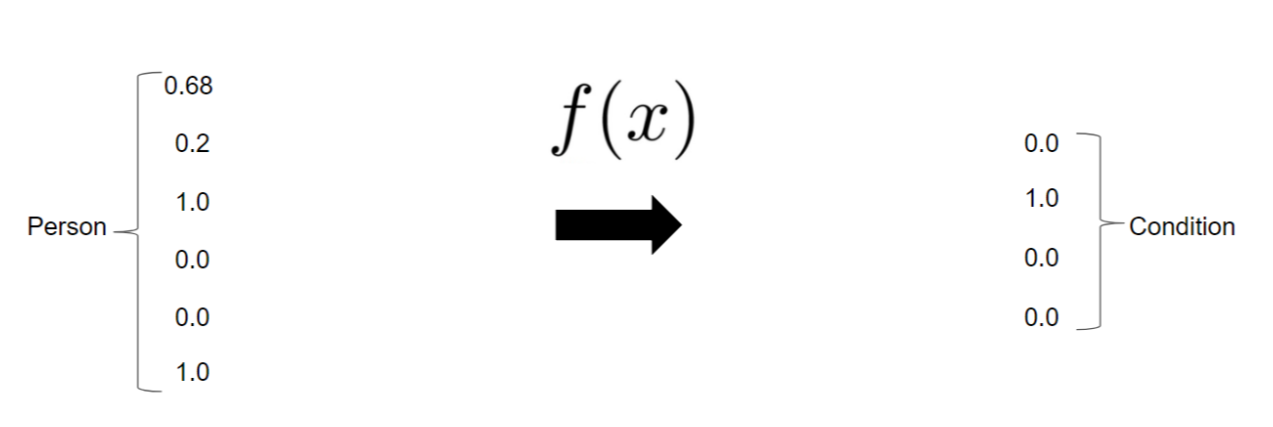
\includegraphics[width=\linewidth]{fgv.png}
  \caption{Általános nézet}
\end{figure}

Ez így elég egyszerűen hangzik, mivel még nem tárgyaltunk arról, hogy ez a függvény hogyan működik, és honnan tud néhány adatból betegségre vonatkozó következtetéseket levonni. A kérdés tehát, hogy hogyan határozzuk meg ezt a függvényt. Legyen a függvény egy neurális háló:

A neurális háló tulajdonképpen egy súlyozott gráf, melynek n darab csúcsa a bemeneteket reprezentálja, k darab csúcsa pedig a kimeneteket. Az n és k csúcsok halmazát rendre input és output layernek (rétegnek) nevezzük, azonban a maradék csúcsok több kisebb halmazra bonthatóak, az úgynevezett hidden (rejtett) rétegekre. 

Egy egyszerű neurális háló tehát L darab layerből áll, melyek közül az input és output layerek speciális funkciót látnak el. A rétegeknek van egy rögzített sorrendje, amely egy neurális hálónak fix tulajdonsága, sosem változik meg. Sorrendben az első réteg az input layer, amit néhány rejtett réteg követ, majd egy output layer zárja a listát.

Minden réteget neuronok egy halmaza alkot. Ezek a gráf csúcsai. Az élek kizárólag a szomszédos layerek neuronja között vannak, méghozzá bármely kettő között pontosan egy él. Tehát az egymással szomszédos rétegek teljes páros gráfot alkotnak együtt. A gráf összes éléhez tartozik egy súly amely minden esetben egy 0 és 1 közé eső szám.

A neuronoknak van egy úgynevezett aktivációs értékük minden pillanatban ami egy 0 és 1 közé eső szám. Egy neuron aktivációs értéket úgy határozzuk meg, hogy vesszük a neuron rétegét megelőző layer azon neuronjait, amelyekkel össze van kötve, majd vesszük ezeknek a lineáris kombinációját a hozzájuk tartozó élek súlyaival. Ehhez még hozzáadunk egy bias értéket, amely magához a vizsgált neuronhoz tartozik és szintén egy 0 és 1 közé eső skalár.
Ezután még az így kapott összegre alkalmazunk egy úgynevezett aktivációs függvényt, amely ugyancsak a neuronhoz tartozik (bár általában egy rétegben minden ez neuronra azonos).

\begin{figure}[h!]
  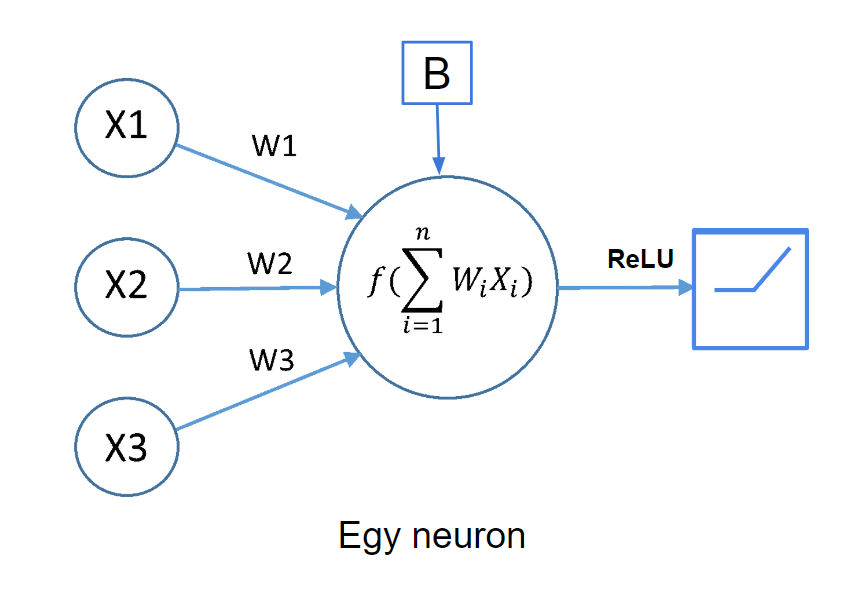
\includegraphics[width=\linewidth]{neuron.png}
  \caption{Egy neuron}
\end{figure}

Az aktivációs függvény rendeltetése, hogy a lineáris kombináció és a bias hozzáadása után keletkezett - várhatóan 1-nél nagyobb - számot visszaskálázzuk a [0-1] intervallumba.
Többféle aktivációs függvény is használhatunk. Gyakoriak:


\subsection{Next}

Lorem ipsum

\end{document}
